% Author: Mark G.

\subsubsection{Description/additional circuitry}
% Describe how your electronic hardware brake plausibility system works (this is in addition to your ECU controlled brake plausibility software), provide tables with main operation parameters, and describe additional circuitry used to check or for an implausibility. Describe how the system reacts if an implausibility or error is detected.

BSPD is represented by a PCB with an on-board current transducer. Brake state signal is received via wiring from ECUP. Output controls Gate of a MOSFET, that acts as a “normally-closed” switch in SDC loop. In case of a trip event output changes state and gets latched till a GLVMS restart.

\begin{table}[H]
	\centering
	\caption{BSPD data}
	\begin{tabularx}{\textwidth}{|X|X|}
		\hline
		Brake sensor used: & Piezoresistive Pressure Transmitter PA-21Y / 100bar / 81691.1 \\[\TableSize]
		\hline
		Brake sensor physical response value: & Voltage, 4,5V \\[\TableSize]
		\hline
		Tractive system power sensor type & Current Transducer LEM HTFS 200-P \\[\TableSize]
		\hline
		Tractive system sensor physical response value: & Voltage of 85mV \\[\TableSize]
		\hline
		Tractive System power sensor current treshold (5kW/Nominal TS voltage): & 14A \\[\TableSize]
		\hline
		Supply voltages: & 5V \\[\TableSize]
		\hline
		Maximum supply currents: & 22mA \\[\TableSize]
		\hline
		Operating temperature: & -40..105$\circ$C\\[\TableSize]
		\hline
		Output used to control AIRs: & Open a MOSFET in SDC \\[\TableSize]
		\hline
	\end{tabularx}%
	\label{tab:addlabel}%
\end{table}%

\begin{figure}[H]
	\centering
	
\includegraphics[width=\textwidth]{./img/bspd-position.jpg}
	\caption{BSPD flowchart.}
	\label{fig:BSPD-flowchart}
\end{figure}

\subsubsection{Schematic}
Describe the wiring, show schematics including the circuit board, show data regarding the cables and connectors used

\begin{figure}[H]
	\centering
	
\includegraphics[width=\textwidth]{./img/bspd-position.jpg}
	\caption{Connection with the SDC schematic.}
	\label{fig:BSPD-conn}
\end{figure}

\subsubsection{Connection with shutdown circuit}

\begin{figure}[H]
	\centering
	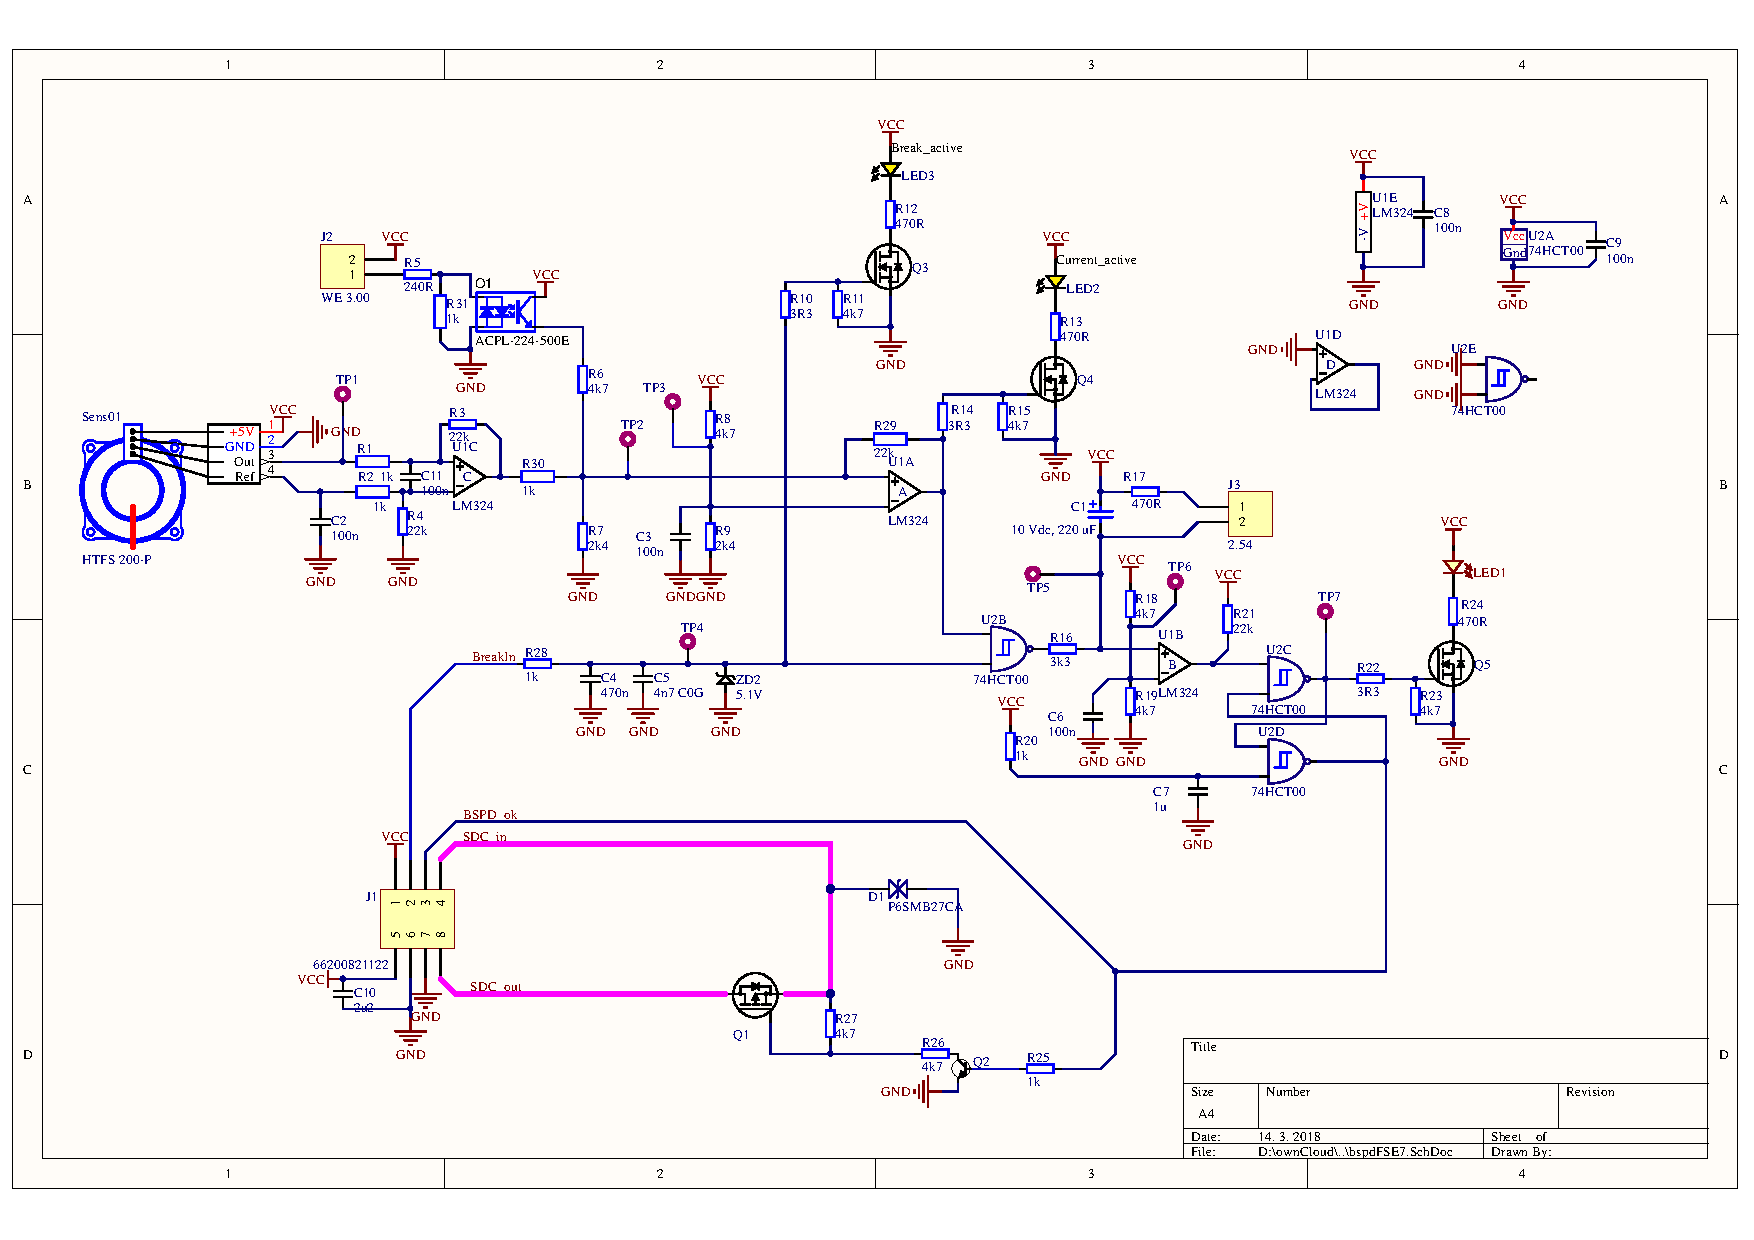
\includegraphics[width=\textwidth]{./img/bspd-schematic.pdf}
	\caption{BSPD schematic sheet.}
	\label{fig:BSPD-schematic}
\end{figure}

\subsubsection{Position in car/mechanical fastening/mechanical connection}
Provide CAD-renderings showing all relevant parts and discuss the mechanical connection of the sensors to the pedal assembly. Mark the parts in the rendering, if necessary.

\begin{figure}[H]
	\centering
	
\includegraphics[width=.5\textwidth]{./img/bspd-position.jpg}
	\caption{BSPD position}
	\label{fig:BSPD-position}
\end{figure}
